\documentclass[margin = 10pt]{standalone} 
\usepackage{tikz}
\usepackage{pgfplots}
\pgfplotsset{compat = 1.18}

\begin{document}
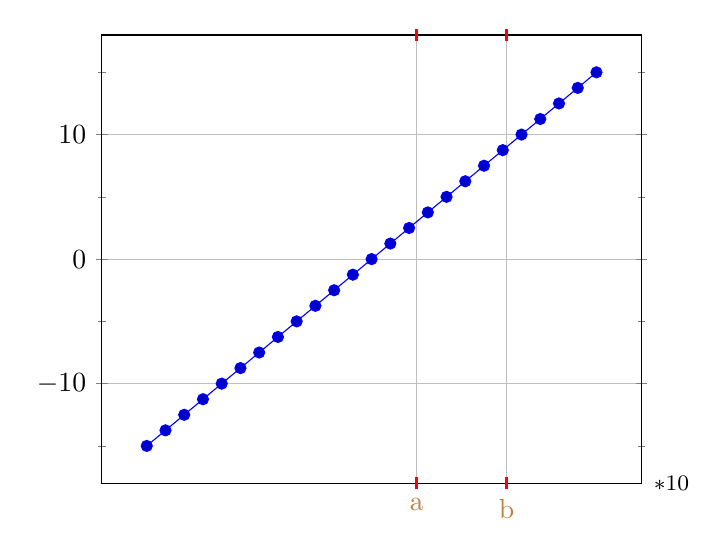
\begin{tikzpicture}[remember picture]
\begin{axis}[
    grid,
    enlargelimits = 0.1,
    % 刻度范围(影响长度)
    % xmin = -4,
    % ymin = -100,
    % xmax = 4,
    % ymax = 100,
    % 
    % 刻度(仅影响显示)
    % xtickmin = -3,
    % ytickmin = -50,
    % xtickmax = 3,
    % ytickmax = 50,
    % 
    % 刻度数值
    % 空
    % xtick= \empty,
    % 自动分配
    xtick= {\empty},
    % 从数据中加载
    % xtick= data,
    % 特殊指定
    % xtick= {1,2,3,4},
    % 
    % 特殊指定子刻度
    % minor xtick={},
    minor xtick={0.5,2.4,3.6,4.8},
    % 设置子刻度数量
    minor z tick num=3,
    minor x tick num=2,
    minor y tick num=1,
    % minor xtick= data,
    % 
    % scaled ticks = real:10,
    % 对齐
    % inside | center | outside
    tick align = center,
    % xtick align = center,
    % 
    % 样式设置
    % tick style = {line width = 10pt},
    % xtick style = {red,line width = 1pt},
    minor x tick style={blue,line width = 1pt},
    major x tick style={red,line width = 1pt},
    % xyz轴同样设置
    % 
    % 
    % 特殊指定刻度
    extra x ticks={1,3},
    % extra x tick label={},
    extra x tick labels={a,b},
    extra x tick style={brown,line width=0.3pt},
    % 
    % 
    % 设置坐标轴缩放比例
    % scaled ticks = real:10,
    scaled x ticks = real:10,
    xtick scale label code/.code={\footnotesize $*10$},
    x tick scale label style={
        at = {(xticklabel* cs:1.022,0)},
        anchor=west,
        }
    ]
    
\addplot   {x*3};
\end{axis}
\end{tikzpicture}
\end{document}